\documentclass[tikz]{standalone}

\usetikzlibrary{mindmap}

\begin{document}
	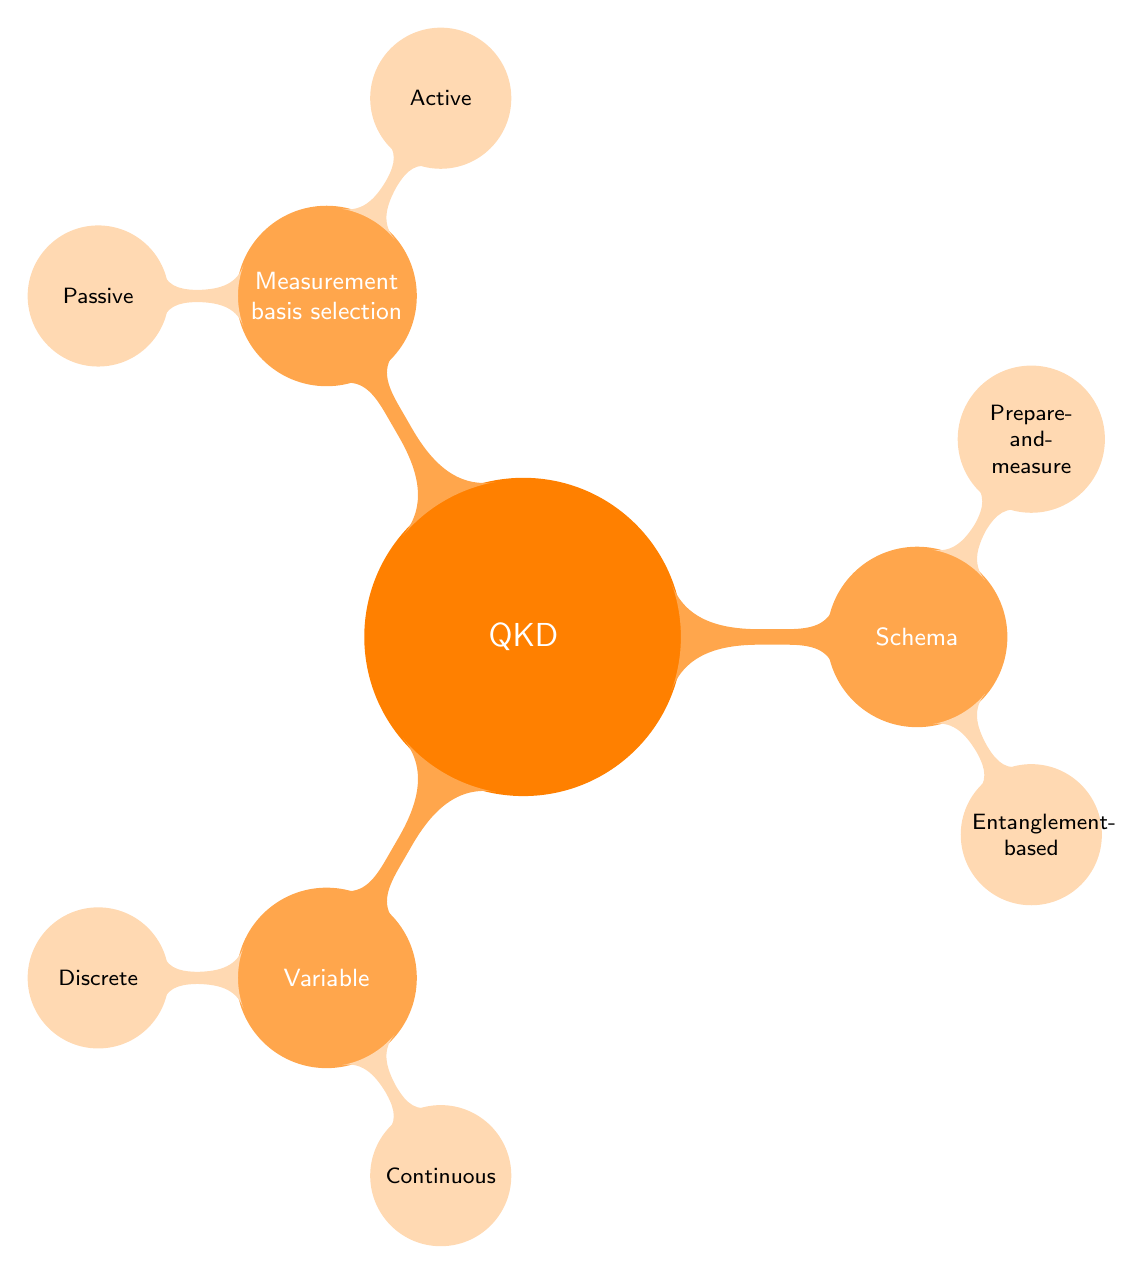
\begin{tikzpicture}[
		mindmap,
		grow cyclic,
		concept color=orange,
		level 1/.append style={
			concept color=orange!70,
			sibling angle=120,
		},
		level 2/.append style={
			concept color=orange!30,
			sibling angle=120,
		},
		every node/.style={
			concept,
		},
	]
		\node[text=white] {\textsf{QKD}}
			child { node[text=white] {\textsf{Variable}}
				child { node {\textsf{Discrete}} }
				child { node {\textsf{Continuous}} }
			}
			child { node[text=white] {\textsf{Schema}}
				child { node {\textsf{Entanglement-based}} }
				child { node {\textsf{Prepare-and-measure}} }
			}
			child { node[text=white] {\textsf{Measurement basis selection}}
				child { node {\textsf{Active}} }
				child { node {\textsf{Passive}} }
			}
		;
	\end{tikzpicture}
\end{document}
